\documentclass[letterpaper,11pt]{article}
\oddsidemargin -1.0cm \textwidth 17.5cm

\usepackage[utf8]{inputenc}
\usepackage[activeacute,spanish, es-lcroman]{babel}
\decimalpoint
\usepackage{amsfonts,setspace}
\usepackage{amsmath}
\usepackage{amssymb, amsmath, amsthm}
\usepackage{comment}
\usepackage{float}
\usepackage{amssymb}
\usepackage{dsfont}
\usepackage{anysize}
\usepackage{multicol}
\usepackage{enumerate}
\usepackage{graphicx}
\usepackage[left=1.5cm,top=2cm,right=1.5cm, bottom=1.7cm]{geometry}
\setlength\headheight{1.5em} 
\usepackage{fancyhdr}
\usepackage{multicol}
\usepackage{hyperref}
\usepackage{wrapfig}
\usepackage{subcaption}
\usepackage{siunitx}
\usepackage{cancel}
\usepackage{mdwlist}
\usepackage{svg}
\pagestyle{fancy}
\fancyhf{}
\renewcommand{\labelenumi}{\normalsize\bfseries P\arabic{enumi}.}
\renewcommand{\labelenumii}{\normalsize\bfseries (\alph{enumii})}
\renewcommand{\labelenumiii}{\normalsize\bfseries \roman{enumiii})}


\begin{document}

\fancyhead[L]{\itshape{Facultad de Ciencias F\'isicas y Matem\'aticas}}
\fancyhead[R]{\itshape{Universidad de Chile}}
\rfoot[]{pág. \thepage}

\begin{minipage}{11.5cm}
    \begin{flushleft}
        \hspace*{-0.6cm}\textbf{FI1100 Introducción a la Física Moderna}\\
        % \hspace*{-0.6cm}\textbf{Tutor:} Alejandro Cartes
    \end{flushleft}
\end{minipage}

\begin{picture}(2,3)
    \put(366, -10){
\includegraphics[scale=0.9]{Imágenes/logo/dfi-fcfm.pdf}}
\end{picture}

\begin{center}
	\LARGE\textbf{Tutoría C3}\\
\end{center}

\vspace{-1cm}
\begin{enumerate}\setlength{\itemsep}{0.4cm}

\item[]

% \item Una cuña de aire se forma entre dos placas de vidrio separadas
% por un alambre muy fino. Cuando la cuña es iluminada desde arriba por una luz de $\SI{600}{\nm}$ y se observa desde arriba, aparecen 30 franjas oscuras. Calcule el radio del alambre

% \begin{figure}[H]
%     \centering
%     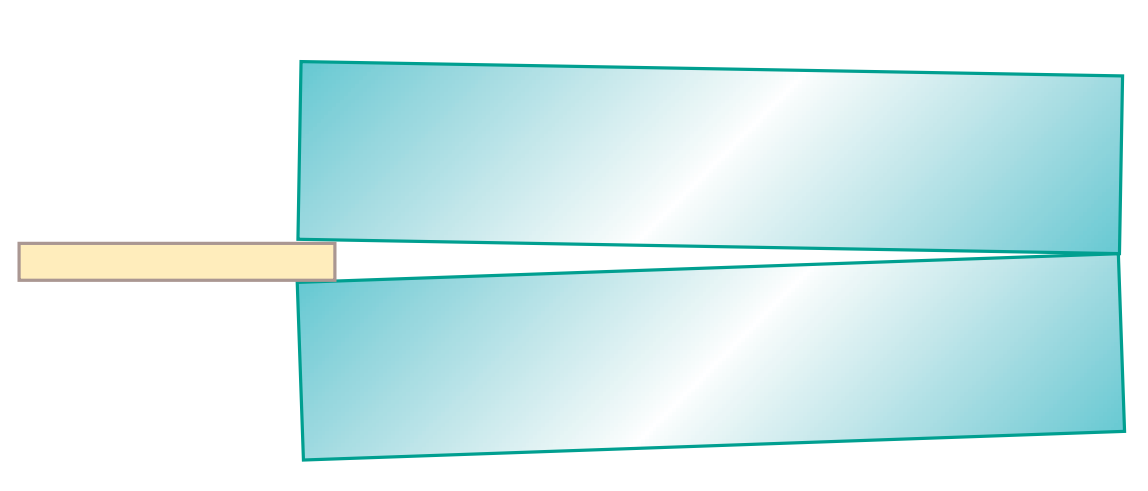
\includegraphics[width=0.25\linewidth]{Imágenes/clases/placas2.png}
% \end{figure}

\item 
\begin{enumerate}
    \item Se observa que en una rendija de apertura $a=\SI{0.8}{\mm}$ ocurre difracción de tal manera que la segunda franja brillante está a una distancia $y=\SI{1.40}{\mm}$ del centro. Si la pantalla está a una distancia $L=\SI{80}{\cm}$, determine la longitud de onda de la luz incidente.

    \item Determine el ancho angular del espectro visible en el primer y tercer orden  que produce una rejilla plana de $600$ ranuras por milímetro cuando incide luz blanca en dirección normal. Considere que las longitudes de ondas del espectro visible abarcan desde $\SI{400}{\nm}$ hasta $\SI{700}{\nm}$
\end{enumerate}

\item La frecuencia media emitida por una bombilla eléctrica de $\SI{200}{\W}$ es $5.00\cdot 10^{14}\SI{}{Hz}$, y el $10\%$ de la potencia se emite como luz visible. ¿Cuántos fotones de luz visible se emiten por segundo?

\item ¿Cuál es la cantidad mínima de energía que se debe transmitir a un átomo de hidrógeno en su nivel fundamental para que pueda emitir la línea $H_{\alpha}$ de la serie de Balmer?

% \item La \textit{Creación de Pares} es un fenómeno en el cual un fotón se transforma en un par partícula-antipartícula, ambas con la misma masa. Por otro lado, la \textit{Aniquilación de Pares}, el par partícula-antipartícula se aniquila y su energía se transforma en un fotón.

% \begin{enumerate}
%     \item Considere un fotón de frecuencia angular $\omega$ el cual se transforma en un par partícula-antipartícula. Si las partículas producidas quedan en reposo y solo poseen energía dada su masa ($E=mc^2$), ¿cuál es la masa de cada partícula?

%     \item Si ahora las partículas producidas caen desde una altura $h$, ¿cuál es la energía del sistema? Si en el suelo el par se aniquila, ¿cuál es la frecuencia del fotón resultante?

%     \item Si ahora mandamos el fotón resultante a la misma altura $h$, para evitar la creación de energía, el fotón debe sufrir una pérdida de energía, de tal manera de crear el par partícula-antipartícula con la misma masa determinada. ¿Cuál debe ser esta pérdida de energía? ¿Cuál es el cambio de frecuencia? 
% \end{enumerate}
% P9: https://strings.lums.edu.pk/home/wp-content/uploads/2015/02/Assignment_3_Solution.pdf

% \item Muestre que la frecuencia de un fotón emitido por un átomo de hidrógeno debido a una transición del electrón de un nivel $n+1$ a $n$ siempre está acotado entre las frecuencias de revolución del electrón en el respectivo nivel orbital
% P4.29: https://fields.sogang.ac.kr/fields/Lecture/Documents/u2013f/documents/solution_4.pdf

\item Considere un nuevo modelo de átomo el cual utiliza la Ley de Hooke $\vec{F} = -kr$ como interacción entre protón y electrón. Usando los postulados de cuantización de Bohr y utilizando órbitas circulares

\begin{enumerate}
    \item Calcule los radios de órbita permitidos

    \item ¿Cuáles son las correspondientes velocidades?

    \item ¿Cuáles son las correspondientes energías?

    \item Determine una expresión análoga a la fórmula de Rydberg
\end{enumerate}

% \item Considere un átomo hidrogenoide en su estado basal cuyo número atómico $Z$ es desconocido. Un fotón es absorbido por este átomo, causando que el electrón se excite hasta un nivel $n$ desconocido. Después de un tiempo, el átomo emite dos fotones sucesivamente. El primer fotón emitido se observó con una longitud de onda de $\SI{434}{\nm}$ y el segundo fotón de $\SI{121}{\nm}$. Si de este átomo se sabe que el segundo fotón emitido corresponde a una transición de $n=2$ a $n=1$

% \begin{enumerate}
%     \item ¿Cuál fue el nivel energético $n$ de excitación?
%     \item ¿Cuál fue la longitud de onda del fotón absorbido?
%     \item ¿Cuál es el valor de $Z$?
% \end{enumerate}

\item Una mujer de pie sobre una escalera deja caer granitos de arena hacia un objetivo puntual en el piso. Demuestre que, según el principio de incertidumbre, la distancia promedio de error debe ser por lo menos
$$\Delta x_f = \left(\frac{2 \hbar}{m}\right)^{1/2}\left(\frac{2H}{g}\right)^{1/4}$$

donde $H$ es la altura inicial de cada granito desde el piso y $m$ es la masa de cada granito. Suponga que la dispersión en los puntos de impacto está dada por $\Delta x_f = \Delta x_i + \Delta v_x t$

% Para imágenes vectoriales -> el texto tiene que estar en LaTeX
% \begin{figure}[htbp]
%   \centering
%   \svgpath{../Imagenes/ejercicios}  -> .. irse pa'trás 
%   \includesvg{ej5.svg}
% \end{figure}

\end{enumerate}
\end{document}
